\documentclass[11pt]{article}
\usepackage{amsmath}
\usepackage{booktabs}
\usepackage[margin=1in]{geometry}
\usepackage{graphicx}
\usepackage{microtype}
\usepackage{tabularx}
\usepackage[hidelinks]{hyperref}

% Archived 147-pair pilot specificity diagnostic macros cited in Section 2
% (single-side control rates from the pre-expansion development pilot).
\newcommand{\GroupedAppropriateFalse}{10/10 = 100.0\%}
\newcommand{\GroupedLinearFalse}{0/5 = 0.0\%}
\newcommand{\GroupedQuadraticFalse}{5/5 = 100.0\%}

% Auto-generated from verified expansion analysis receipt (do not hand-edit).
% Manifest SHA-256: 5b432d827f324c073eb7ed14b4df4b5d18f5eb2a90c4d97d358405a800d27346
% Amendment 5 SHA-256: 17de6626bb871cc30f80040bd63f123da8c0b4498231ff63b607045b36fdb469
\newcommand{\BenchPairs}{1{,}000}
\newcommand{\BenchPIE}{728}
\newcommand{\BenchVal}{500}
\newcommand{\BenchTrain}{228}
\newcommand{\BenchCodeNet}{228}
\newcommand{\BenchGitHub}{44}
\newcommand{\BenchContestPairs}{956}
\newcommand{\BenchGCC}{15.2.0}
\newcommand{\BenchMinClusters}{200}
\newcommand{\BenchMinFits}{30}
\newcommand{\BenchMinSizes}{4}
\newcommand{\BenchMinSpan}{8}
\newcommand{\BenchMinSlope}{0.50}
\newcommand{\BenchMinRatio}{1.50}
\newcommand{\BenchRecovery}{80\%}
\newcommand{\BenchAuthorSample}{50}
\newcommand{\BenchPilotPairs}{147}
\newcommand{\BenchPilotDeskN}{103}
\newcommand{\BenchPilotDeskPct}{70.1\%}
\newcommand{\BenchPilotExecN}{14}
\newcommand{\BenchPilotExecPct}{9.5\%}
\newcommand{\BenchPilotFitN}{13}
\newcommand{\BenchPilotAlertN}{4}
\newcommand{\BenchPilotAlertPct}{30.8\%}
\newcommand{\BenchPilotIntakeAlertPct}{2.7\%}
\newcommand{\BenchPilotPrepN}{12}
\newcommand{\BenchPilotPrepDenom}{26}
\newcommand{\BenchPilotPrepPct}{46.2\%}
\newcommand{\BenchPilotOracleN}{1}
\newcommand{\BenchPilotOraclePct}{7.1\%}
\newcommand{\BenchPilotSAFiveDelta}{$-33.3$~pp}
\newcommand{\BenchCpuCapSec}{8\,s}
\newcommand{\BenchStackCapMB}{8\,\text{MiB}}
\newcommand{\BenchFileCapMB}{8\,\text{MiB}}
\newcommand{\BenchTickCeiling}{$\max(2\times 10^{6},\,5N^{2})$}
\newcommand{\BenchCpuFloorMs}{10\,\text{ms}}
\newcommand{\BenchSpawnFloorMs}{0.5\,\text{ms}}
\newcommand{\BenchCensorTolPct}{10\%}
\newcommand{\BenchBwrapVer}{0.11.1}
\newcommand{\BenchPilotFitClustersN}{12}
\newcommand{\BenchPilotFitClustersFrac}{4/12}
\newcommand{\BenchPilotConservFrac}{3/12}
\newcommand{\BenchPilotNeffThirty}{30}
\newcommand{\BenchPilotNeffFifty}{50}
\newcommand{\BenchPilotNeffRange}{30\text{--}75}
\newcommand{\BenchPosSevenOne}{71}
\newcommand{\BenchPosNineNine}{99}
\newcommand{\BenchPosOneZeroSeven}{107}
\newcommand{\BenchPosOneOneSix}{116}
\newcommand{\BenchPosOneThreeNine}{139}
\newcommand{\BenchPosOneFourOne}{141}
\newcommand{\BenchPosOneSixSeven}{167}
\newcommand{\BenchNumVariants}{4}
\newcommand{\BenchNumModes}{5}
\newcommand{\BenchNumStreams}{3}
\newcommand{\BenchFDWire}{3}
\newcommand{\BenchUbuntuVer}{26.04}
\newcommand{\BenchMemCapMiB}{768\,\text{MiB}}
\newcommand{\BenchTasksCap}{24}
\newcommand{\BenchAsCapMiB}{512\,\text{MiB}}
\newcommand{\BenchWallCapSec}{12\,\text{s}}
\newcommand{\BenchCompileTimeoutSec}{25\,\text{s}}
\newcommand{\BenchTickExitCode}{85}
\newcommand{\BenchPilotExecUpperPct}{15.5\%}
\newcommand{\BenchOLSMinRSq}{0.6584}
\newcommand{\BenchRestTwoSidedBand}{80--120\%}
\newcommand{\BenchCensorSlopeMin}{0.45}
\newcommand{\BenchWaveOnePin}{\texttt{04f1a1b2}}
\newcommand{\BenchWaveTwoPin}{\texttt{b598ea21}}
\newcommand{\BenchBetaGridMin}{0.20}
\newcommand{\BenchBetaGridDrop}{0.10}
\newcommand{\BenchRestSurgicalBand}{80--105\%}
\newcommand{\BenchRestMildBand}{105--120\%}
\newcommand{\BenchRestHighBand}{$>120\%$}
\newcommand{\BenchPinManifest}{\texttt{5b432d82}}
\newcommand{\BenchPinProtocol}{\texttt{8a969245}}
\newcommand{\BenchPinHolds}{\texttt{6bc97dea}}
\newcommand{\BenchPinAmendFive}{\texttt{17de6626}}
\newcommand{\BenchPinAnon}{\texttt{c2ba8209}}
\newcommand{\BenchPinForensics}{\texttt{b8ea9b8c}}
\newcommand{\BenchSlot}[1]{\textnormal{[\emph{#1}:~\rule{1.3em}{0.35pt}]}}
\newcommand{\BenchCell}{\textnormal{[\rule{1.3em}{0.35pt}]}}
\newcommand{\BenchIntakeStopsN}{23}
\newcommand{\BenchIntakeDupN}{12}
\newcommand{\BenchIntakeUnretN}{11}
\newcommand{\BenchIntakeContestN}{12}
\newcommand{\BenchIntakeRepoN}{11}
\newcommand{\BenchSOPassN}{977}
\newcommand{\BenchQuarPairsN}{500}
\newcommand{\BenchQuarClustersN}{54}
\newcommand{\BenchConfPairsN}{477}
\newcommand{\BenchConfClustersN}{476}
\newcommand{\BenchConfContestClustersN}{444}
\newcommand{\BenchConfRepoClustersN}{32}
\newcommand{\BenchConfRepoPairsN}{33}
\newcommand{\BenchConfSingletonN}{475}
\newcommand{\BenchConfRepoSingletonN}{31}
\newcommand{\BenchHeldUnratAllN}{133}
\newcommand{\BenchRepoDeskUnratN}{33}
\newcommand{\BenchContestUnbundledConfN}{86}
\newcommand{\BenchHeldUnratConfClustN}{118}
\newcommand{\BenchHeldConfPairsN}{119}
\newcommand{\BenchRateablePairsN}{844}
\newcommand{\BenchSOneBatchesN}{96}
\newcommand{\BenchSOneAttemptsN}{102}
\newcommand{\BenchSOneRetriesN}{6}
\newcommand{\BenchSOneDateWindow}{2026-11-23, 04:09--10:09~UTC}
\newcommand{\BenchFittedClusters}{124}
\newcommand{\BenchExecRate}{149/476 = 31.3\% (95\% CP 27.2--35.7\%)}
\newcommand{\BenchDeskContrast}{+30.3~pp across 476 clusters (95\% cluster bootstrap +22.1 to +38.4~pp, Holm $p_H = 2.03 \times 10^{-11}$)}
\newcommand{\BenchPOneCount}{149}
\newcommand{\BenchPOnePct}{31.3\%}
\newcommand{\BenchPOneCI}{[27.2, 35.7]\%}
\newcommand{\BenchPOneHolmP}{$p = 1.97 \times 10^{-39}$}
\newcommand{\BenchPOneFisherP}{$p = 2.73 \times 10^{-8}$}
\newcommand{\BenchPTwoDelta}{+30.3~pp}
\newcommand{\BenchPTwoHolmP}{$p = 6.78 \times 10^{-12}$}
\newcommand{\BenchPTwoHoldsPP}{+24.8~pp}
\newcommand{\BenchPTwoHoldsShare}{81.9\%}
\newcommand{\BenchPTwoRateableContribPP}{+5.5~pp}
\newcommand{\BenchPThreeCount}{6}
\newcommand{\BenchPThreePct}{4.8\%}
\newcommand{\BenchPThreeCI}{[1.8, 10.2]\%}
\newcommand{\BenchPThreeHolmP}{$p = 2.53 \times 10^{-12}$}
\newcommand{\BenchPThreeFisherP}{$p = 0.0076$}
\newcommand{\BenchSAFiveSignP}{$p = 4.42 \times 10^{-28}$}
\newcommand{\BenchSATwoPct}{1.3\%}
\newcommand{\BenchSATwoCI}{[0.5, 2.7]\%}
\newcommand{\BenchSATwoFisherP}{$p = 0.257$}
\newcommand{\BenchRateableClustersN}{358}
\newcommand{\BenchRateableExecPct}{41.6\%}
\newcommand{\BenchRateableExecCI}{[36.5, 46.9]\%}
\newcommand{\BenchRateableDeskPct}{48.9\%}
\newcommand{\BenchSAThirteenDelta}{+7.3~pp}
\newcommand{\BenchSAThirteenBootCI}{[$-2.8$, +17.0]~pp}
\newcommand{\BenchSAThirteenP}{$p = 0.165$}
\newcommand{\BenchConfSTwoPassN}{183}
\newcommand{\BenchRatedDeskStopRepsN}{175}
\newcommand{\BenchTotalDeskStopRepsN}{293}
\newcommand{\BenchConfContractStopRepsN}{160}
\newcommand{\BenchConfSourceStopRepsN}{11}
\newcommand{\BenchConfRouteStopRepsN}{2}
\newcommand{\BenchConfIndetRepsN}{2}
\newcommand{\BenchFixtureStopN}{32}
\newcommand{\BenchFixtureStopPct}{17.5\%}
\newcommand{\BenchFixtureStopCI}{[12.3, 23.8]\%}
\newcommand{\BenchCondExecPct}{81.4\%}
\newcommand{\BenchOrigCompileFailN}{4}
\newcommand{\BenchOrigCompileFailPct}{2.2\%}
\newcommand{\BenchOrigCompileFailCI}{[0.6, 5.5]\%}
\newcommand{\BenchRunnerSOnePassN}{154}
\newcommand{\BenchRunnerPreFixtureN}{29}
\newcommand{\BenchRunnerOverlayFixtureN}{3}
\newcommand{\BenchOracleFailN}{17}
\newcommand{\BenchOracleFailPct}{11.4\%}
\newcommand{\BenchOracleFailCI}{[6.8, 17.6]\%}
\newcommand{\BenchNoFitN}{8}
\newcommand{\BenchNoAlertN}{118}
\newcommand{\BenchInfraFailN}{2}
\newcommand{\BenchQuarUnrunN}{204}
\newcommand{\BenchPinLedger}{\texttt{59dcfaf3}}
\newcommand{\BenchPinRepPlan}{\texttt{99c0b425}}
\newcommand{\BenchConfContestDrawn}{456}
\newcommand{\BenchConfContestIntake}{12}
\newcommand{\BenchQuarIntakeN}{0}
\newcommand{\BenchQuarPostSOneZeroN}{0}
\newcommand{\BenchConfContestDesk}{261}
\newcommand{\BenchConfContestFix}{32}
\newcommand{\BenchConfContestPrep}{0}
\newcommand{\BenchConfContestInfra}{2}
\newcommand{\BenchConfContestUnrun}{0}
\newcommand{\BenchConfContestOracle}{17}
\newcommand{\BenchConfContestNoFit}{8}
\newcommand{\BenchConfContestNoAlert}{118}
\newcommand{\BenchConfContestAlert}{6}
\newcommand{\BenchQuarContestDesk}{296}
\newcommand{\BenchBwrapOverheadMs}{14--22\,\text{ms}}
\newcommand{\BenchWaveOneOverrideN}{6}
\newcommand{\BenchPinWaveTwoCap}{\texttt{1c926287}}
\newcommand{\BenchPosNineFourPlainUpperNs}{0.35}
\newcommand{\BenchPosTwoNine}{29}
\newcommand{\BenchPosNineZeroOZeroOnlyPts}{2}
\newcommand{\BenchPosNineSevenOtwoStreamsN}{1}
\newcommand{\BenchPosNineSevenPlainStreamsN}{0}
\newcommand{\BenchPosThirteenPlainStreamsFrac}{2/3}
\newcommand{\BenchPosThirteenOtwoStreamsFrac}{3/3}
\newcommand{\BenchPosOneSevenFivePlainStreamsFrac}{3/3}
\newcommand{\BenchPosOneSevenFiveOtwoStreamsFrac}{3/3}
\newcommand{\BenchPosOneSixFourPlainStreamsFrac}{0/3}
\newcommand{\BenchPosOneSixFourOtwoStreamsFrac}{0/3}
\newcommand{\BenchPosNineFourPlainStreamsFrac}{0/3}
\newcommand{\BenchPosNineFourOtwoStreamsFrac}{0/3}
\newcommand{\BenchPosNineSevenPlainStreamsFrac}{0/3}
\newcommand{\BenchMaxCounterVal}{$2.50 \times 10^{9}$}
\newcommand{\BenchUnconfRestoredOracleN}{0}
\newcommand{\BenchFittedMaskedFailN}{0}
\newcommand{\BenchPosOneSixFourTotSlopeTwoDec}{0.00}
\newcommand{\BenchPosThreeWorstTS}{0.00}
\newcommand{\BenchAllPtMaxBoundFailN}{0}
\newcommand{\BenchMinRefPlainCoreN}{2}
\newcommand{\BenchMinRefOtwoCoreN}{2}
\newcommand{\BenchMedRefPlainCoreN}{1}
\newcommand{\BenchMedRefOtwoCoreN}{2}
\newcommand{\BenchAddCpuOneThreeSlopeRange}{6.45--9.97}
\newcommand{\BenchAddCpuOneSevenFiveSlopeRange}{17.45--118.25}
\newcommand{\BenchAddCpuOneSixFourSlopeRange}{7.01--7.54}
\newcommand{\BenchAddCpuNineFourSlopeRange}{$-1.31$ to 0.84}
\newcommand{\BenchAddCpuNineSevenSlopeRange}{0.08--1.77}
\newcommand{\BenchOtwoMinusPlainSZeroMs}{0.75\,\text{ms} median, IQR 0.36--1.52\,\text{ms}}
\newcommand{\BenchRestNonExSATwoN}{2}
\newcommand{\BenchRestNonExSubN}{1}
\newcommand{\BenchRestNonExFlatN}{5}
\newcommand{\BenchRestNonExNegN}{4}
\newcommand{\BenchRestNonExMixN}{2}
\newcommand{\BenchAllPtExcessFailN}{0}
\newcommand{\BenchAllPtRoneInflN}{0}
\newcommand{\BenchAllPtNonRegFailN}{2}
\newcommand{\BenchPosEighteen}{18}
\newcommand{\BenchPosFourFour}{44}
\newcommand{\BenchPOnePilotNeffTipN}{19}
\newcommand{\BenchOZeroAgree}{9{,}794}
\newcommand{\BenchOZeroMiss}{1{,}294}
\newcommand{\BenchOZeroTotalTriples}{11{,}088}
\newcommand{\BenchOZeroCapped}{40}
\newcommand{\BenchOZeroOracleAbort}{1{,}138}
\newcommand{\BenchOZeroOverlayFix}{112}
\newcommand{\BenchOZeroInfraMiss}{4}
\newcommand{\BenchOZeroCapOtwoAgree}{12}
\newcommand{\BenchShamAgree}{7{,}349}
\newcommand{\BenchShamMiss}{967}
\newcommand{\BenchShamTotalPairs}{8{,}316}
\newcommand{\BenchShamCapped}{35}
\newcommand{\BenchShamOracleAbort}{855}
\newcommand{\BenchShamOverlayFix}{75}
\newcommand{\BenchShamInfraMiss}{2}
\newcommand{\BenchCpuCapEvents}{28}
\newcommand{\BenchCpuCapPos}{3}
\newcommand{\BenchTickCapEvents}{72}
\newcommand{\BenchTickCapPos}{2}
\newcommand{\BenchCpuCapOZeroOnlyPts}{5}
\newcommand{\BenchCpuCapTotalPts}{7}
\newcommand{\BenchOracleUpstreamN}{16}
\newcommand{\BenchOracleUpstreamPct}{10.7\%}
\newcommand{\BenchOracleUpstreamCI}{[6.3, 16.9]\%}
\newcommand{\BenchOracleUpstreamTgtN}{10}
\newcommand{\BenchOracleUpstreamRefN}{6}
\newcommand{\BenchOraclePlainN}{12}
\newcommand{\BenchOraclePlainUpstreamN}{11}
\newcommand{\BenchOraclePlainTgtN}{8}
\newcommand{\BenchOraclePlainRefN}{3}
\newcommand{\BenchOracleUBAllN}{5}
\newcommand{\BenchOracleUBSanOnlyN}{4}
\newcommand{\BenchOracleUBTgtN}{2}
\newcommand{\BenchOracleUBRefN}{3}
\newcommand{\BenchOraclePlainSegvUBN}{1}
\newcommand{\BenchOracleRestoredN}{1}
\newcommand{\BenchOracleShamN}{0}
\newcommand{\BenchOracleMultiEvtN}{2}
\newcommand{\BenchOracleCoordN}{6}
\newcommand{\BenchOracleCoordPct}{35.3\%}
\newcommand{\BenchFitQZeroN}{2}
\newcommand{\BenchFitBothZeroN}{4}
\newcommand{\BenchFitTickCapN}{2}
\newcommand{\BenchCensorCondN}{7}
\newcommand{\BenchCensorDenom}{126}
\newcommand{\BenchCensorCondPct}{5.6\%}
\newcommand{\BenchCensorCondCI}{[2.3, 11.1]\%}
\newcommand{\BenchCensorWorstN}{8}
\newcommand{\BenchCensorWorstPct}{6.3\%}
\newcommand{\BenchCensorWorstCI}{[2.8, 12.1]\%}
\newcommand{\BenchCensorWorstFisherP}{$p = 0.015$}
\newcommand{\BenchCensorWorstFisherFourTwelveP}{$p = 0.011$}
\newcommand{\BenchCensorWorstFisherConservP}{$p = 0.056$}
\newcommand{\BenchCensorCpuCapExclFlatN}{9}
\newcommand{\BenchCensorCpuCapExclFlatPct}{7.1\%}
\newcommand{\BenchCensorCpuCapExclFlatP}{$p = 0.021$}
\newcommand{\BenchCensorCpuCapExclFlatConservP}{$p = 0.071$}
\newcommand{\BenchCensorCpuCapTotalN}{11}
\newcommand{\BenchCensorCpuCapPct}{8.7\%}
\newcommand{\BenchCensorCpuCapFourTwelveP}{$p = 0.027$}
\newcommand{\BenchCensorCpuCapConservP}{$p = 0.106$}
\newcommand{\BenchJointConservHolmPOne}{$p_H = 0.026$}
\newcommand{\BenchJointConservHolmPThree}{$p_H = 0.033$}
\newcommand{\BenchDistinctThreeN}{70}
\newcommand{\BenchDistinctThreePct}{56.5\%}
\newcommand{\BenchDistinctTwoN}{9}
\newcommand{\BenchDistinctTwoPct}{7.3\%}
\newcommand{\BenchDistinctOneN}{45}
\newcommand{\BenchDistinctOnePct}{36.3\%}
\newcommand{\BenchDistinctOneCOneVarN}{12}
\newcommand{\BenchDistinctOneOblivN}{33}
\newcommand{\BenchZeroVarStreamsN}{171}
\newcommand{\BenchDefinedRTwoStreamsN}{201}
\newcommand{\BenchTotalFittedStreamsN}{372}
\newcommand{\BenchAllStreamsMedianRTwo}{0.864}
\newcommand{\BenchAlertMedianRTwo}{0.9999}
\newcommand{\BenchZeroVarPairsN}{52}
\newcommand{\BenchDefinedRTwoPairsN}{72}
\newcommand{\BenchPairMedianRTwo}{0.738}
\newcommand{\BenchAlertPairMedianRTwo}{0.9994}
\newcommand{\BenchPThreePilotClustFisherP}{$p = 0.0056$}
\newcommand{\BenchPThreePilotClustConservP}{$p = 0.033$}
\newcommand{\BenchPOnePilotNeffThirtyP}{$p = 0.013$}
\newcommand{\BenchPOnePilotNeffFiftyP}{$p = 9.70 \times 10^{-4}$}
\newcommand{\BenchSAOnePilotNeffRangeP}{$p = 0.157\text{--}0.439$}
\newcommand{\BenchSAThreeInclCompileN}{4}
\newcommand{\BenchSAThreeInclCompilePct}{2.2\%}
\newcommand{\BenchSAThreeInclCompileP}{$p = 1.27 \times 10^{-9}$}
\newcommand{\BenchSAThreeCrossFrameP}{$p = 5.82 \times 10^{-12}$}
\newcommand{\BenchConstZeroVarPairsN}{6}
\newcommand{\BenchCensorCpuCapFisherP}{$p = 0.035$}
\newcommand{\BenchRestCOneMaskN}{2}
\newcommand{\BenchSANinePThreeCI}{[1.6, 8.9]\%}
\newcommand{\BenchOZeroRelaxCapPtsN}{5}
\newcommand{\BenchOZeroRelaxPairsN}{3}
\newcommand{\BenchOZeroRelaxDeltaN}{0}
\newcommand{\BenchRealizedCpuCoreN}{2}
\newcommand{\BenchPlainSubCoreN}{1}
\newcommand{\BenchOtwoSubCoreN}{2}
\newcommand{\BenchFDWrapOverheadMs}{0.78\,\text{ms} median, IQR $-0.04$ to 1.81\,\text{ms}}
\newcommand{\BenchPosOneSixFourCpuRatio}{2.10--2.20$\times$}
\newcommand{\BenchSubCpuOneSevenFiveSlopeRange}{0.97--1.93}
\newcommand{\BenchSubCpuOneThreeSlopeRange}{0.48--1.02}
\newcommand{\BenchPosThirteenPlainZeroSubRange}{0.61--0.96}
\newcommand{\BenchPosThirteenOtwoSubSlopeRange}{0.72--1.50}
\newcommand{\BenchPosOneSevenFiveOtwoSubSlopeRange}{1.12--1.80}
\newcommand{\BenchPosThirteenPlainDeltaMsRange}{26.5--44.4\,\text{ms}}
\newcommand{\BenchPosOneSevenFivePlainDeltaMsRange}{52.6--490.4\,\text{ms}}
\newcommand{\BenchSubCpuOneSixFourSlopeRange}{$-0.05$ to 0.13}
\newcommand{\BenchSubCpuNineFourSlopeRange}{$-0.55$ to 0.37}
\newcommand{\BenchSubCpuNineSevenSlopeRange}{0.03--0.21}
\newcommand{\BenchSASevenCount}{11}
\newcommand{\BenchSASevenPct}{8.9\%}
\newcommand{\BenchSASevenCI}{[4.5, 15.3]\%}
\newcommand{\BenchSASevenOnlyN}{5}
\newcommand{\BenchSAEightAdmittedN}{123}
\newcommand{\BenchSAEightAlertsN}{5}
\newcommand{\BenchSAEightPct}{4.1\%}
\newcommand{\BenchSAEightCI}{[1.3, 9.2]\%}
\newcommand{\BenchSAEightAnyAlertsN}{10}
\newcommand{\BenchSAEightAnyPct}{8.1\%}
\newcommand{\BenchSAEightAnyCI}{[4.0, 14.4]\%}
\newcommand{\BenchCoreFourN}{4}
\newcommand{\BenchCoreFourPct}{3.2\%}
\newcommand{\BenchCoreFourCI}{[0.9, 8.1]\%}
\newcommand{\BenchCoreMinCILo}{0.97}
\newcommand{\BenchBOneAlertsN}{32}
\newcommand{\BenchBOnePct}{25.8\%}
\newcommand{\BenchBOneCI}{[18.4, 34.4]\%}
\newcommand{\BenchBOneFPN}{26}
\newcommand{\BenchBOneFlatN}{12}
\newcommand{\BenchBOneSubN}{6}
\newcommand{\BenchBOneNegN}{5}
\newcommand{\BenchBOneSelN}{3}
\newcommand{\BenchBOneMcNemarP}{$p = 2.98 \times 10^{-8}$}
\newcommand{\BenchBOneHolmP}{$p = 1.49 \times 10^{-7}$}
\newcommand{\BenchBTwoAlertsN}{7}
\newcommand{\BenchBTwoPct}{5.6\%}
\newcommand{\BenchBTwoCI}{[2.3, 11.3]\%}
\newcommand{\BenchBThreeAlertsN}{5}
\newcommand{\BenchBThreePct}{4.0\%}
\newcommand{\BenchBThreeCI}{[1.3, 9.2]\%}
\newcommand{\BenchBThreeAllExecN}{5}
\newcommand{\BenchBThreeAllExecDenom}{132}
\newcommand{\BenchBThreeAllExecPct}{3.8\%}
\newcommand{\BenchBFourAlertsN}{0}
\newcommand{\BenchBFourPct}{0.0\%}
\newcommand{\BenchBFourCI}{[0.0, 2.9]\%}
\newcommand{\BenchBFourMcNemarP}{$p = 0.031$}
\newcommand{\BenchBFourHolmP}{$p = 0.094$}
\newcommand{\BenchBFiveAlertsN}{17}
\newcommand{\BenchBFivePct}{13.7\%}
\newcommand{\BenchBFiveCI}{[8.2, 21.0]\%}
\newcommand{\BenchBFiveTPN}{3}
\newcommand{\BenchBFiveFPN}{14}
\newcommand{\BenchBFiveMcNemarP}{$p = 0.013$}
\newcommand{\BenchBFiveHolmP}{$p = 0.051$}
\newcommand{\BenchBFiveCoreTPN}{2}
\newcommand{\BenchBFiveCorePrecPct}{11.8\%}
\newcommand{\BenchBFiveCoreRecPct}{50.0\%}
\newcommand{\BenchRestPassAllN}{54}
\newcommand{\BenchRestNoExAllN}{66}
\newcommand{\BenchRestFailAllN}{18}
\newcommand{\BenchRestUnmeasAllN}{45}
\newcommand{\BenchRestExecPassN}{51}
\newcommand{\BenchRestExecNoExN}{65}
\newcommand{\BenchRestExecFailN}{18}
\newcommand{\BenchRestExecUnmeasN}{15}
\newcommand{\BenchRestFitPassN}{47}
\newcommand{\BenchRestFitNoExN}{63}
\newcommand{\BenchRestFitFailN}{14}
\newcommand{\BenchRestFitExcessN}{61}
\newcommand{\BenchRestFitFailPct}{23.0\%}
\newcommand{\BenchRestFitFailCI}{[13.2, 35.5]\%}
\newcommand{\BenchRestExactCopyN}{33}
\newcommand{\BenchRestExactCopyPct}{70.2\%}
\newcommand{\BenchRestNonExactPassN}{14}
\newcommand{\BenchRestSurgicalN}{9}
\newcommand{\BenchRestMildOverN}{3}
\newcommand{\BenchRestHighOverN}{2}
\newcommand{\BenchRestTotPassN}{62}
\newcommand{\BenchRestTotNoExN}{49}
\newcommand{\BenchRestTotFailN}{13}
\newcommand{\BenchRestTotExcessN}{75}
\newcommand{\BenchRestTotFailPct}{17.3\%}
\newcommand{\BenchRestTotFailCI}{[9.6, 27.8]\%}
\newcommand{\BenchRestTotNewTestN}{14}
\newcommand{\BenchConfDeskPairsN}{294}
\newcommand{\BenchFinHolmPOne}{$p_H = 5.45 \times 10^{-8}$}
\newcommand{\BenchFinHolmPThree}{$p_H = 0.0076$}
\newcommand{\BenchCOneOnlyCount}{2}
\newcommand{\BenchPosEleven}{11}
\newcommand{\BenchPosElevenCOneStream}{\texttt{W3}}
\newcommand{\BenchPosFourSevenCOneStream}{\texttt{W2}}
\newcommand{\BenchPosElevenCOneRatio}{13.8$\times$}
\newcommand{\BenchQOneZeroCount}{10}
\newcommand{\BenchPosThreeLev}{0.524}
\newcommand{\BenchPosThreeCooksD}{2.20}
\newcommand{\BenchPosThreeCooksDSThree}{0.52}
\newcommand{\BenchPosThreeCooksDSThreeMax}{0.73}
\newcommand{\BenchPosThreeSOneLOO}{0.00}
\newcommand{\BenchPosThreeSThreeLOO}{$-0.43$}
\newcommand{\BenchPosThreeSOneCI}{[-0.65, 2.82]}
\newcommand{\BenchPosThreeSThreeCI}{[-2.90, 4.21]}
\newcommand{\BenchPosThirteenCZeroSlope}{2.01}
\newcommand{\BenchPosThirteenTotSlope}{1.02}
\newcommand{\BenchPosNineFourOtwoNsRange}{0.03--0.06}
\newcommand{\BenchPosNineFourPlainNsRange}{$-0.20$ to +0.34}
\newcommand{\BenchPosNineFourOtwoMsRange}{1.1--1.9\,\text{ms}}
\newcommand{\BenchPosOneSevenFiveOtwoNsRange}{7.5--23.7}
\newcommand{\BenchPosOneSevenFivePlainNsRange}{4.5--19.6}
\newcommand{\BenchEnvPOneRange}{30.0--31.7\%}
\newcommand{\BenchEnvPThreeRange}{4.8--5.0\%}
\newcommand{\BenchEnvSAFourRange}{7.7--11.6\%}
\newcommand{\BenchEnvSAThirteenRange}{+6.7~pp ($p = 0.203$) to +8.9~pp ($p = 0.082$)}
\newcommand{\BenchEnvSAThirteenShort}{+6.7 to +8.9~pp, $p = 0.082\text{--}0.203$}
\newcommand{\BenchPfStderrN}{1}
\newcommand{\BenchPfSigabrtN}{2}
\newcommand{\BenchPfSigsegvN}{4}
\newcommand{\BenchRegimeExactEqN}{46}
\newcommand{\BenchRegimeFlatLowN}{24}
\newcommand{\BenchRegimeFlatHighN}{12}
\newcommand{\BenchRegimeZeroFlatSumN}{82}
\newcommand{\BenchRegimeNegAllN}{13}
\newcommand{\BenchRegimeMixedN}{10}
\newcommand{\BenchRegimeSubPosN}{8}
\newcommand{\BenchRegimeRevSubSumN}{31}
\newcommand{\BenchBetaGridDropAlerts}{10}
\newcommand{\BenchCorpusPieAlertFrac}{3/69}
\newcommand{\BenchCorpusCodeAlertFrac}{3/55}
\newcommand{\BenchCorpusAlertFisherP}{$p = 1.000$}
\newcommand{\BenchCorpusPieExecFrac}{84/228 = 36.8\%}
\newcommand{\BenchCorpusCodeExecFrac}{65/216 = 30.1\%}
\newcommand{\BenchCorpusExecFisherP}{$p = 0.159$}
\newcommand{\BenchContestExecPct}{33.6\%}
\newcommand{\BenchContestExecCI}{[29.2, 38.2]\%}
\newcommand{\BenchContestExecLo}{29.2\%}
\newcommand{\BenchSAFourFisherP}{$p = 1.000$}
\newcommand{\BenchSAThreeDenom}{154}
\newcommand{\BenchSAThreeAllSPass}{0/183 = 0.0\%}
\newcommand{\BenchSAThreeAllSPassCI}{[0.0, 2.0]\%}
\newcommand{\BenchPosThreeRSq}{0.061}
\newcommand{\BenchPosSevenSevenLogRSq}{1.000}
\newcommand{\BenchPosOneSixFourRatio}{20{,}001$\times$}
\newcommand{\BenchPosOneSixFourTotP}{$p = 0.013$}
\newcommand{\BenchPosOneSixFourTotSlope}{0.0002}
\newcommand{\BenchPosOneSixFourTotRSq}{0.821}
\newcommand{\BenchPosSevenNine}{79}
\newcommand{\BenchPosSevenNineSlopeRange}{0.97--0.99}
\newcommand{\BenchPosSevenNineRatioRange}{0.79--0.91$\times$}
\newcommand{\BenchQuarSourceN}{25}
\newcommand{\BenchQuarHeldN}{14}
\newcommand{\BenchQuarIndetN}{1}
\newcommand{\BenchRestCOneInflN}{0}
\newcommand{\BenchPosThree}{3}
\newcommand{\BenchPosThirteen}{13}
\newcommand{\BenchPosTwoSeven}{27}
\newcommand{\BenchPosFourSeven}{47}
\newcommand{\BenchPosFiveFive}{55}
\newcommand{\BenchPosFiveNine}{59}
\newcommand{\BenchPosSevenSeven}{77}
\newcommand{\BenchPosNineZero}{90}
\newcommand{\BenchPosNineOne}{91}
\newcommand{\BenchPosNineFour}{94}
\newcommand{\BenchPosNineSeven}{97}
\newcommand{\BenchPosOneZeroZero}{100}
\newcommand{\BenchPosOneZeroSix}{106}
\newcommand{\BenchPosOneTwoNine}{129}
\newcommand{\BenchPosOneThreeOne}{131}
\newcommand{\BenchPosOneFourZero}{140}
\newcommand{\BenchPosOneFourFive}{145}
\newcommand{\BenchPosOneFiveEight}{158}
\newcommand{\BenchPosOneSixZero}{160}
\newcommand{\BenchPosOneSixFour}{164}
\newcommand{\BenchPosOneSevenFour}{174}
\newcommand{\BenchPosOneSevenFive}{175}
\newcommand{\BenchPosSevenSevenRatio}{7.86$\times$}
\newcommand{\BenchPosNineZeroRatio}{23{,}899$\times$}
\newcommand{\BenchPosOneFourFiveRatio}{134$\times$}
\newcommand{\BenchPosFourSevenCOneRatio}{492$\times$}
\newcommand{\BenchPosNineFourTicksM}{32.0}
\newcommand{\BenchPosOneSixFourTotRatio}{2.00$\times$}
\newcommand{\BenchPosOneZeroZeroMaxSlope}{0.075}
\newcommand{\BenchPosBothZeroMaxSlope}{0.013}
\newcommand{\BenchRestOverNineOneRange}{121--146\%}
\newcommand{\BenchRestOverOneTwoNineRange}{103--315\%}
\newcommand{\BenchQuarStopPct}{59.2\%}
\newcommand{\BenchQuarStopCI}{[54.7, 63.5]\%}
\newcommand{\BenchQuarClustStopFrac}{32/54 = 59.3\%}
\newcommand{\BenchQuarClustStopCI}{[45.0, 72.4]\%}
\newcommand{\BenchAuthExactPct}{26.0\%}
\newcommand{\BenchAuthExactK}{0.163}
\newcommand{\BenchAuthExactCI}{[0.046, 0.277]}
\newcommand{\BenchAuthBucketPct}{48.0\%}
\newcommand{\BenchAuthBucketK}{0.154}
\newcommand{\BenchAuthBucketCI}{[$-0.031$, 0.326]}
\newcommand{\BenchAuthBucketKappaMax}{0.479}
\newcommand{\BenchAuthBucketACOne}{0.271}
\newcommand{\BenchAuthBinPct}{56.0\%}
\newcommand{\BenchAuthBinK}{0.032}
\newcommand{\BenchAuthBinPABAK}{0.120}
\newcommand{\BenchAuthBinACOne}{0.263}
\newcommand{\BenchAuthBinBI}{0.32}
\newcommand{\BenchAuthBinPI}{0.44}
\newcommand{\BenchAuthBowkerQ}{16.40}
\newcommand{\BenchAuthMcNemarP}{$p = 8.55 \times 10^{-4}$}
\newcommand{\BenchAuthBowkerP}{$p = 9.39 \times 10^{-4}$}
\newcommand{\BenchAuthAllBowkerExactP}{$p = 1.55 \times 10^{-4}$}
\newcommand{\BenchAuthConfN}{20}
\newcommand{\BenchAuthQuarN}{30}
\newcommand{\BenchAuthQuarClustersN}{18}
\newcommand{\BenchAuthTotalClustersN}{38}
\newcommand{\BenchAuthLLMPassFrac}{22/50 = 44.0\%}
\newcommand{\BenchAuthAuthorPassFrac}{6/50 = 12.0\%}
\newcommand{\BenchAuthConfPct}{30.0\%}
\newcommand{\BenchAuthConfKappa}{0.018}
\newcommand{\BenchAuthConfBinK}{$-0.170$}
\newcommand{\BenchAuthConfBucketKCI}{[$-0.231$, 0.265]}
\newcommand{\BenchAuthConfBinKCI}{[$-0.500$, 0.186]}
\newcommand{\BenchAuthConfPABAKCI}{[$-0.500$, 0.300]}
\newcommand{\BenchAuthConfACOneCI}{[$-0.467$, 0.483]}
\newcommand{\BenchAuthConfAllStopRev}{3/11 = 27.3\%}
\newcommand{\BenchAuthConfAllStopRevCI}{[6.0, 61.0]\%}
\newcommand{\BenchAuthConfPassStopN}{8}
\newcommand{\BenchAuthConfStopPassN}{3}
\newcommand{\BenchAuthConfMcNemarP}{$p = 0.227$}
\newcommand{\BenchAuthConfBowkerQ}{8.00}
\newcommand{\BenchAuthConfBowkerP}{$p = 0.046$}
\newcommand{\BenchAuthConfBowkerExactP}{$p = 0.041$}
\newcommand{\BenchAuthQuarPct}{60.0\%}
\newcommand{\BenchAuthQuarKappa}{0.259}
\newcommand{\BenchAuthQuarBinK}{0.171}
\newcommand{\BenchAuthQuarRev}{0/16 = 0.0\%}
\newcommand{\BenchAuthCohortFisherP}{$p = 0.048$}
\newcommand{\BenchCohortClustSensP}{$p = 0.101\text{--}0.188$}
\newcommand{\BenchAuthConfContractRev}{3/10 = 30.0\%}
\newcommand{\BenchAuthConfContractRevCI}{[6.7, 65.2]\%}
\newcommand{\BenchAuthRejExec}{7/8~=~87.5\%}
\newcommand{\BenchAuthRejExecCI}{[47.3, 99.7]\%}
\newcommand{\BenchAuthPassStopN}{19}
\newcommand{\BenchAuthStopPassN}{3}
\newcommand{\BenchAuthRejTotalN}{8}
\newcommand{\BenchManskiTipNum}{13}
\newcommand{\BenchManskiTipRate}{7.4\%}
\newcommand{\BenchManskiPlugInTheta}{22.2\%}
\newcommand{\BenchManskiPlugInThetaCI}{[4.9, 49.6]\%}
\newcommand{\BenchManskiPlugJointRectCI}{[4.5, 52.9]\%}
\newcommand{\BenchManskiPlugJointJeffCI}{[6.8, 46.1]\%}
\newcommand{\BenchManskiPlugInSAThirteen}{$-14.4$~pp}
\newcommand{\BenchManskiPlugInTwoStepSAThirteen}{$-16.9$~pp}
\newcommand{\BenchManskiPlugInPOne}{52.5\%}
\newcommand{\BenchManskiFullFlipTheta}{41.1\%}
\newcommand{\BenchManskiTwoStepTipTheta}{6.7\%}
\newcommand{\BenchManskiTwoStepTipPfn}{8.2\%}
\newcommand{\BenchManskiYOneStepHalfPP}{1.6~pp}
\newcommand{\BenchManskiYTwoStepHalfPP}{0.8~pp}
\newcommand{\BenchManskiYDeltaSEDiffPP}{0.03~pp}
\newcommand{\BenchPThreeOracleTipN}{9}
\newcommand{\BenchPThreeOracleTipPct}{52.9\%}
\newcommand{\BenchPThreeOracleTipResultPct}{10.6\%}
\newcommand{\BenchPThreeOracleTipConservN}{3}
\newcommand{\BenchPThreeOracleTipConservPct}{17.6\%}
\newcommand{\BenchPThreeOracleAdvTipN}{8}
\newcommand{\BenchPThreeOracleAdvTipPct}{47.1\%}
\newcommand{\BenchPThreeOracleAdvTipConservN}{2}
\newcommand{\BenchPThreeOracleAdvTipConservPct}{11.8\%}
\newcommand{\BenchPThreeSOneTipN}{8}
\newcommand{\BenchPThreeSOneTipPct}{4.6\%}
\newcommand{\BenchPThreeSOneTipResultPct}{10.6\%}
\newcommand{\BenchPThreeSOneTipConservN}{2}
\newcommand{\BenchPThreeSOneTipConservPct}{1.1\%}
\newcommand{\BenchSAThirteenFpTipN}{6}
\newcommand{\BenchSAThirteenFpTipPct}{4.0\%}
\newcommand{\BenchSAThirteenFpTipDelta}{+10.6~pp}
\newcommand{\BenchSAThirteenFpTipP}{$p = 0.040$}
\newcommand{\BenchAuthConfFitRejFrac}{6/7 = 85.7\%}
\newcommand{\BenchPThreeFpTipConservN}{20}
\newcommand{\BenchPThreeFpTipConservPct}{16.9\%}
\newcommand{\BenchPThreeFpTipConservP}{$p = 0.050$}
\newcommand{\BenchPThreeFpTipFullN}{57}
\newcommand{\BenchPThreeFpTipFullPct}{48.3\%}
\newcommand{\BenchPThreeFpTipFullP}{$p = 0.052$}
\newcommand{\BenchTableTwoRows}{\textbf{P1}\,$^{\ddagger}$ & Execution yield (conf.\ reps) & 149/476 (31.3\%) & [27.2, 35.7]\% & Holm & $5.45 \times 10^{-8}$ & 1-S $1.97 \times 10^{-39}$ \\ \textbf{P2} & Desk stop $-$ execution & +30.3~pp (476 cl.) & [+22.1, +38.4]~pp & Holm & $2.03 \times 10^{-11}$ & exact sign; hold+WF \\ \quad $\hookrightarrow$ & Unrateable holds share & +24.8~pp (81.9\%) & --- & --- & --- & --- \\ \quad $\hookrightarrow$ & Rateable Contest contrib. & +5.5~pp (18.1\%) & --- & --- & --- & --- \\ \textbf{P3} & All-stream alerts / fits & 6/124 (4.8\%) & [1.8, 10.2]\% & Holm & $0.0076$ & 1-S $2.53 \times 10^{-12}$ \\ \midrule \textbf{SA1} & Desk stops (conf.\ reps) & 293/476 (61.6\%) & [57.0, 65.9]\% & Fisher\,$^\dagger$ & $0.063$ & 1-S $7.39 \times 10^{-5}$ \\ \textbf{SA2} & Alerts / post-S0 conf.\ reps & 6/476 (1.3\%) & [0.5, 2.7]\% & Fisher\,$^\dagger$ & $0.257$ & 1-S $0.048$ \\ \textbf{SA3}\,$^{\ddagger}$ & S2 preprocessing stops & 0/154 (0.0\%) & [0.0, 2.4]\% & --- & --- & x-frame (4/183 comp.) \\ \textbf{SA4} & Oracle / UBSan failures & 17/149 (11.4\%) & [6.8, 17.6]\% & Fisher\,$^\dagger$ & $1.000$ & env.\ 7.7--11.6\% \\ \textbf{SA5} & Alert $-$ no-alert (vs.\ 50\%) & $-90.3$~pp (124 fits) & [$-96.8$, $-82.3$]~pp & Sign & $4.42 \times 10^{-28}$ & vs.\ $-33.3$~pp pilot \\ \textbf{SA6} & P1 excl.\ infra stops & 149/474 (31.4\%) & [27.3, 35.8]\% & --- & --- & 2 infra excl. \\ \textbf{SA7} & Any-stream alerts / fits & 11/124 (8.9\%) & [4.5, 15.3]\% & --- & --- & any-stream \\ \textbf{SA8} & Drop-largest all-stream & 5/123 (4.1\%) & [1.3, 9.2]\% & --- & --- & 1 range-lim. \\ \textbf{SA9} & Equal-cluster P1 (all pairs) & 31.3\% (476 cl.) & [27.1, 35.5]\% & --- & --- & boot.; P3 [1.6, 8.9]\% \\ \textbf{SA10} & Contest P1 (within-Contest) & 149/444 (33.6\%) & [29.2, 38.2]\% & --- & --- & 32 Repo held at S1 \\ \textbf{SA12} & Quarantined S1 stops (cl.) & 32/54 (59.3\%) & [45.0, 72.4]\% & --- & --- & 59.2\% pairs; 204 unrun \\ \textbf{SA13a} & Rateable Contest P1 & 149/358 (41.6\%) & [36.5, 46.9]\% & --- & --- & excl.\ 118 holds \\ \textbf{SA13b} & Rateable Contest P2 & +7.3~pp (358 cl.) & [$-2.8$, +17.0]~pp & Sign & $0.165$ & toggles 0.082--0.203 \\ \textbf{SA14} & Pre-S3 fixture stops & 32/183 (17.5\%) & [12.3, 23.8]\% & --- & --- & cond.\ 81.4\% \\}
\newcommand{\BenchAlertForensicsRows}{3 (CodeNet) & 32--1{,}024 (3/3) & 0.65--2.24 & $-2.90$/0.00 & 193--1{,}119$\times$ & 0.69--2.24 & 193--1{,}119$\times$ & Flip & 0.99--1.04$\times$ & $\times$ & $\times$ \\ 13 (CodeNet) & 50--1{,}600 (1/3) & 2.01 & 2.00/2.01 & 2.56\text{M}$\times$ & 1.02 & 3{,}193$\times$ & Retain & 2.00--3.69$\times$ & \checkmark & \checkmark \\ 94 (PIE) & 250--8{,}000 (1/3) & 1.00 & 1.00/1.00 & 4{,}000$\times$ & 1.01 & 3{,}066--3{,}983$\times$ & Retain & 0.79--1.48$\times$ & \checkmark & $\times$ \\ 97 (PIE) & 1--32 (3/3) & 1.86--1.93 & 1.29/1.91 & 394--413$\times$ & 1.87--1.96 & 408--426$\times$ & Retain & 1.10--1.15$\times$ & \checkmark & $\times$ \\ 164 (PIE) & 625--20{,}000 (1/3) & 1.00 & 1.00/1.00 & 20{,}001$\times$ & 0.00 & 2.00$\times$ & Retain & 2.10--2.20$\times$ & $\times$ & \checkmark \\ 175 (CodeNet) & 300--9{,}600 (3/3) & 0.99--1.05 & 0.97/0.99 & 1{,}221--2{,}763$\times$ & 0.99--1.04 & 611--1{,}382$\times$ & Retain & 3.07--22.65$\times$ & \checkmark & \checkmark \\}
\newcommand{\BenchTableFourRows}{Overall (38 cl.) & 50 & 48.0\% (0.154; [$-0.031$, 0.326]) & 56.0\% (0.032) & 0.120 & 0.263 & 3/19/3/25 & 3/26 & ($8.55 \times 10^{-4}$)\,$^\dagger$ \\ Conf.\ (sing.) & 20 & 30.0\% (0.018; [$-0.231$, 0.265]) & 45.0\% ($-0.170$) & $-0.100$ & 0.020 & 1/8/3/8 & 3/10 & $0.227$\phantom{$\,^\dagger$} \\ Quar.\ (18 cl.) & 30 & 60.0\% (0.259; ---) & 63.3\% (0.171) & 0.267 & 0.413 & 2/11/0/17 & 0/16 & ($9.77 \times 10^{-4}$)\,$^\dagger$ \\}
\newcommand{\BenchTableCorpusRows}{PIE-train (Contest) & 228 & 228 & 46 & 83 & 99 & 15 & 0 & 84 & 9 & 6 & 69 & 3 \\ CodeNet (Contest) & 228 & 216 & 40 & 92 & 84 & 17 & 2 & 65 & 8 & 2 & 55 & 3 \\ GitHub (Repository) & 44 & 33 & 33 & 0 & 0 & 0 & 0 & 0 & 0 & 0 & 0 & 0 \\ \midrule \textbf{Total} & 500 & 477 & 119 & 175 & 183 & 32 & 2 & 149 & 17 & 8 & 124 & 6 \\}
\newcommand{\BenchTableAppRows}{Primary protocol baseline (SHA \texttt{59dcfaf3}) & 31.3\% & +30.3~pp & +7.3~pp ($0.165$) & 4.8\% & 11.4\% & 17.5\% \\ Pre-patch \texttt{cpu\_cap} exit-137 (2 pairs; \texttt{1c926287}) & 30.9\% & +30.7~pp & +7.8~pp ($0.132$) & 4.9\% & 11.6\% & 17.5\% \\ All \texttt{cpu\_cap} exit-137 unpatched (3 pairs; incl.\ Case~139) & 30.7\% & +30.9~pp & +8.1~pp ($0.118$) & 5.0\% & 11.6\% & 17.5\% \\ 8\,MiB stack policy (2 pairs, \texttt{rc=139}) as \texttt{fixture\_stop} & 31.3\% & +30.3~pp & +7.3~pp ($0.165$) & 4.8\% & 11.4\% & 18.6\% \\ Non-empty \texttt{stderr} diagnostic pairs (2 pairs) as executed & 31.7\% & +29.8~pp & +6.7~pp ($0.203$) & 4.8\% & 11.3\% & 16.4\% \\ Residual UB/crash traps (2 pairs, \texttt{rc=134/139}) as infra & 31.3\% & +30.3~pp & +7.3~pp ($0.165$) & 4.8\% & 11.4\% & 16.4\% \\ Capped-point quality toggle (1 pair as \texttt{insufficient\_fit}) & 31.3\% & +30.3~pp & +7.3~pp ($0.165$) & 4.9\% & 11.4\% & 17.5\% \\ Initial-batch oracle overrides (6 pairs) as \texttt{fixture\_stop} & 30.0\% & +31.5~pp & +8.9~pp ($0.082$) & 4.8\% & 7.7\% & 20.8\% \\}
\newcommand{\BenchFlowIntakeC}{12}
\newcommand{\BenchFlowIntakeR}{11}
\newcommand{\BenchFlowIntakeU}{23}
\newcommand{\BenchFlowDeskC}{557}
\newcommand{\BenchFlowDeskR}{33}
\newcommand{\BenchFlowDeskU}{590}
\newcommand{\BenchFlowFixtureC}{32}
\newcommand{\BenchFlowFixtureR}{0}
\newcommand{\BenchFlowFixtureU}{32}
\newcommand{\BenchFlowPrepC}{0}
\newcommand{\BenchFlowPrepR}{0}
\newcommand{\BenchFlowPrepU}{0}
\newcommand{\BenchFlowInfraC}{2}
\newcommand{\BenchFlowInfraR}{0}
\newcommand{\BenchFlowInfraU}{2}
\newcommand{\BenchFlowUnrunC}{204}
\newcommand{\BenchFlowUnrunR}{0}
\newcommand{\BenchFlowUnrunU}{204}
\newcommand{\BenchFlowOracleC}{17}
\newcommand{\BenchFlowOracleR}{0}
\newcommand{\BenchFlowOracleU}{17}
\newcommand{\BenchFlowNoFitC}{8}
\newcommand{\BenchFlowNoFitR}{0}
\newcommand{\BenchFlowNoFitU}{8}
\newcommand{\BenchFlowNoAlertC}{118}
\newcommand{\BenchFlowNoAlertR}{0}
\newcommand{\BenchFlowNoAlertU}{118}
\newcommand{\BenchFlowAlertC}{6}
\newcommand{\BenchFlowAlertR}{0}
\newcommand{\BenchFlowAlertU}{6}


\title{When Can a C++ Performance Pair Support a Growth Claim?\\
An Empirical Study of Benchmark Qualification}
\author{Anonymous authors}
\date{November 2026}
\hypersetup{pdftitle={When Can a C++ Performance Pair Support a Growth Claim?},
  pdfauthor={Anonymous authors}}

\begin{document}
\maketitle

\begin{abstract}
A faster C++ program is a candidate for a growth benchmark, not evidence
that the original program's work increases faster with input size.
We study \BenchPairs{} frozen public slow--fast pairs from PIE, CodeNet, and
GitHub performance fixes. A frozen protocol follows each pair from intake
through model-based desk screening, a sandboxed build, an independent output
oracle, and a fit to the ratio of counts of a shared work event. The
execution yield was \BenchExecRate, and the all-stream alert rate was
\BenchFitAlertRate{} among fitted representatives and \BenchIntakeAlertRate{}
among representatives passing intake. \BenchAbstractTakeaway{} A screen pass
concerns the named event on the tested inputs, not time complexity or
elapsed time. Confirmatory inference on fitted-case alerts requires at least
\BenchMinFits{} independent fitted clusters (satisfied here with 124 fits).
\end{abstract}

\noindent\textbf{Keywords:} benchmark qualification, software performance,
empirical growth, program instrumentation, C++.

\section{Introduction}

Performance-improvement datasets provide program versions ordered by some
notion of speed. In contest data that ordering can come from timings on a
judge's fixed tests; in a repository it may come from a developer's claim in a
commit message. Neither ordering tells us whether the programs perform the same
task on new inputs, whether they expose the same measurable operation, or
whether the input range permits a comparison of growth. Even a large decrease
in work at one size can be a constant-factor change. Conversely, a pair that
cannot be built in isolation may still be useful in its own project. Treating
these cases as failed growth tests, or dropping them before reporting a
denominator, obscures what a benchmark can support.

We ask how many public slow--fast C++ pairs can support a finite-range
growth claim under one specified execution route. The study distinguishes
three questions: How often does a comparison reach isolated execution (P1)?
Is the rate of desk stops higher or lower than the rate of reaching execution
when problems and projects receive equal weight (P2)? Among comparisons
that admit a fit, how often does the work ratio pass the growth
screen (P3)? We also report alerts per intake-passing representative so the
conditional fitted-case rate is not mistaken for overall yield. Desk labels
are model judgments, not ground truth; a blind check by one author is
separate. Fewer than \BenchMinFits{} fitted clusters permits a descriptive
account, not a directional claim about fitted-case yield.

Our contribution is an accounting of where and why pairs stop, from the
frozen manifest to a fit or a documented terminal disposition. We separate
contest submissions from project patches and keep development-exposed
comparisons out of the confirmatory estimates. The outcome of applying the
protocol is \BenchIntroTakeaway. A high yield would show that the tested
route supports measurement for many pairs in these frames; a low yield
would identify which prerequisites constrain it. Neither outcome establishes
that the underlying optimizations are or are not worthwhile.

\section{Related work}

PIE uses execution performance to identify improvement examples for learning
code edits~\cite{shypula2024pie}. Project-based collections such as
CppPerf mine performance edits together with build or test
context~\cite{ho2026cppperf}. Such resources answer how to obtain candidate
comparisons; we ask what can be measured after selection. As with other uses
of mined GitHub data, the metadata and the collection route delimit the
population to which the results apply~\cite{kalliamvakou2014promises}.
Test-backed benchmarks such as Defects4J illustrate the value of a checked
witness~\cite{just2014defects4j}; here at least one scalable workload and a
common operation are needed in addition to checks of output.

Empirical computational complexity measures work as the input size
varies~\cite{goldsmith2007measuring}. We fit a ratio for the same event in
two versions, on the same inputs, and qualify the resulting claim to the
measured range. This avoids treating compiler-dependent timing as a direct
measure of a single operation, but does not remove the need to control the
environment~\cite{mytkowicz2009producing}. Instrumentation and build choices
can still change the program or the set of feasible comparisons.

\paragraph{Development evidence.}
The archived paired audit motivated tracking desk stops separately from
execution and distinguishing admissible fits from alerts. It was a
development sample with inherited controls, not an estimate from the
expanded frame. In a separate replay-only diagnostic, false-alert rates
were \GroupedQuadraticFalse{} for quadratic same-growth shams,
\GroupedLinearFalse{} for linear same-growth shams, and
\GroupedAppropriateFalse{} for appropriate superlinear controls.
The pilot evidence does not support ranker superiority. Neither set of
pilot results is pooled with the benchmark under study.

\section{Study design}
\label{sec:design}

\subsection{Frozen intake and independent units}

The manifest fixes \BenchPairs{} pair identities before benchmark execution.
PIE supplies \BenchPIE{} rows (\BenchVal{} validation and \BenchTrain{}
training); CodeNet~\cite{puri2021codenet}
supplies \BenchCodeNet{}, and GitHub performance-fix commits supply
\BenchGitHub{}. The PIE test split is not used.
The \emph{Contest} frame contains the PIE and CodeNet submissions. PIE
supplies the released timing order. The CodeNet draw uses consecutive
accepted C++ submissions from the same author, problem, and compiler
language, with a strictly lower positive judge CPU time on the later
submission; submissions already used in PIE are excluded from this draw.
For the \emph{Repository} frame, the candidate reference is a public
commit whose subject says it fixes performance, and the target is its
parent. These labels establish an orientation, not a measured speed
ordering on our workloads.

The extension uses a bounded repository search and hash-ordered contest
draw. It takes one contest pair per problem in the extension, skipping
problems already drawn, and alternates between PIE training and CodeNet while
both have eligible clusters. CodeNet is restricted to PIE training problems
so that no test-split metadata is needed. The repository snapshot and its
page expansion are documented in the intake record. Selection does not
prefer pairs that look easier to build or likely to pass. Each row carries
its upstream pin and available source hashes. Retrieval or licence failures
and duplicates remain visible as intake stops, rather than being replaced.

A row is a pair; a test unit is a connected component. Initial keys are
judge and problem for contest submissions and upstream repository root for
patches. Shared aliases, normalized source, and identifier- and
literal-normalized template matches connect keys, including across frames.
Pairs in components linked to the archived audit and the retained
development-exposed validation stratum do not enter the confirmatory
analysis. Missing fingerprint evidence is not evidence of no overlap.
The analysis reports Contest, Repository, and their distinct union; the
union counts a shared pair once. After intake and quarantine, a stable
hash of the corpus, component, and pair identifiers selects the
representative before desk inspection, with lexical tie breaking. All
other rows still receive a disposition.

\subsection{Qualification and the run contract}

Each comparison is accounted for at its earliest terminal stage. At
\textsc{S0} we check retrieval at the pinned identities, C++ source, usable
licence evidence, and uniqueness. Intake failures are reported against the
frozen manifest but excluded from analysis rates. At \textsc{S1} the desk
assessment asks whether the pair supports a legal six-size geometric
ladder on three workload streams, an independent oracle, a countable
event with the same meaning in both versions, and an isolated restoration
and sham edit. Source findings
such as an output defect are distinct from missing measurement contracts
and from barriers specific to the build route. Four dated protocol
amendments refined Stage~S1 labeling before confirmatory execution:
Amendment~1 assigned \texttt{desk\_unrateable} without model inspection to
packets lacking self-contained specifications and restricted Repository
reporting to counts only; Amendment~2 dropped the second S1 rater;
Amendment~3 classified all S1-dependent rates as \emph{replay-only}; and
Amendment~4 added terminal \texttt{indeterminate} when the primary rater
cannot decide desk criteria. Accordingly, all Repository pairs (whose
commits carry no independent specification) and Contest pairs whose problem
statements reference unbundled images receive \texttt{desk\_unrateable},
and both \texttt{desk\_unrateable} and \texttt{indeterminate} stay in
every post-S0 denominator (counting as desk stops in P2 and as not
reaching execution in P1) and never enter S2 or P3; sensitivity
analysis~S13 repeats P1--P3 with \texttt{desk\_unrateable} removed.
Because every Repository S0-pass pair is \texttt{desk\_unrateable}, no
Repository test runs and the Union equals Contest for every rated or
executed outcome. The logged reason records
which prerequisite stopped the pair, not that either program is slow or
that its growth is negative.

Eligible pairs advance in stable-hash order, not in order of expected
growth. At \textsc{S2} the Gate~1 runner checks dependencies by preprocessing
the comparison as a single translation unit. At \textsc{S3} the target,
reference, restoration, and sham build and run under the Bubblewrap
launcher in the pinned container with GCC~\BenchGCC. The restoration edits
the target to replace the proposed mechanism; the sham is an edit intended
to preserve the measured work. Plain and undefined-behavior-sanitized
outputs must agree with an oracle independent of the pair. Counted builds
must report the same work counts at \texttt{-O0}, \texttt{-O2}, and
\texttt{-O3}. An observed oracle failure and an infrastructure failure have
different implications: the former counts as reaching execution, whereas
the latter does not. Infrastructure retries use the same pins and stop at
the protocol's limit. Pairs not executed at closure are recorded rather
than deferred off the ledger. No post-intake stop is discarded from the
P1 or P2 denominator within the confirmatory frame.

\paragraph{Model judgments and blind check.}
The desk decisions are model-based, not human. \BenchDeskMethods{}
Inter-model agreement was not measured (\BenchModelAgreement).
S1 labels come from one Devin workflow whose backend routing the vendor
does not disclose, so they cannot be reproduced; P1--P3 computed from
them are \emph{replay-only} rather than re-executable (Amendment~3).
Conditional on the fixed S1 passes, S2--S5 Gate~1 preprocessing,
isolated execution, and fitting remain deterministic and
\emph{re-executable} from the pinned fixtures, and P3's
$\ge \BenchMinFits{}$ confirmatory fitted-cluster gate is satisfied.
The separate blind
check covers \BenchAuthorSample{} pairs from a draw frozen before
production labeling and is carried out by one author without access to
model decisions while assigning labels. It is descriptive only, never
establishes human ground truth, and never alters primary labels or
triggers adjudication.

\paragraph{Amendment~5 (\texttt{17de6626}) and execution disclosures.}
Prior to confirmatory S3 execution, Amendment~5 (\texttt{17de6626},
2026-11-23) refined S2--S5 handling from disjoint development evidence
(183/183 confirmatory S2 preprocessing passes under GCC~\BenchGCC{} and
3/5 fixture-authoring stops in a 5-pair quarantined diagnostic):
(i)~an S1 pass failing constructive fixture verification before S3
receives terminal \texttt{fixture\_stop} with a bucket, reason, and
SHA-256-pinned proof, staying in post-S0 denominators as not executed in
P1 and S9, keeping $\text{desk stop}=0$ and $\text{executed}=0$ in P2,
remaining outside P3, and reporting as S14; and
(ii)~confirmatory-only quota-gated execution runs the 183 confirmatory S1
passes in frozen hash order across waves (target $\le 75\%$, hard cap
$80\%$ weekly quota) while recording the 204 quarantined S12 passes and any
unattempted confirmatory tail as \texttt{not\_executed} (reporting frozen
bounds and prefix-conditional yields if truncated at $K < 183$).
Under protocol Section~11, Wave~1--3 operational disclosures are documented
alongside independent sensitivity toggles: \texttt{gate1\_sandbox.py} enforces
\texttt{prlimit --cpu=8:8}, which emits \texttt{SIGKILL} (exit~137)
rather than \texttt{SIGXCPU}; Wave~2's two 8\,s CPU kills
(\texttt{oom\_kill = 0}, \texttt{oom\_group\_kill = 0}) halted at
\texttt{terminal = None} until \texttt{expansion\_run.py} was patched
(\texttt{04f1a1b2}, local commit \texttt{9518f3e2}; Wave~1 baseline
\texttt{1c926287} replayed identically with zero exit-137 rows) to record
non-OOM exit~137/$-9$ at \texttt{cpu.stat.usage\_usec} $\ge 8\times 10^{6}$
as right-censored \texttt{cpu\_cap} and to emit \texttt{insufficient\_fit}
when $<4$ uncapped sizes remain. Under the patched runner, both Wave~2 pairs
re-executed cleanly to admissible \texttt{no\_alert} fits (20 and 4
\texttt{cpu\_cap} events; sensitivity treating both as infrastructure failure
yields P1 $147/476 = 30.9\%$, P2 $+30.7$~pp, P3 $6/122 = 4.9\%$, 95\% CP
$1.8\text{--}10.4\%$). Across all waves, \texttt{cpu\_cap} fired 28 times
across 3 positions: 24 on those two Wave~2 pairs plus 4 on one Wave~3
\texttt{no\_alert} position (position~139, executed directly under patched
runner \texttt{04f1a1b2}; a classification-only rollback to
\texttt{terminal = null} shifts P1 from 149 to 148 and leaves P3 at 6, so
reverting all three \texttt{cpu\_cap} positions together bounds unpatched P1
at $146/476 = 30.7\%$ and P3 at $6/121 = 5.0\%$). Across Waves~2 and~3, five
\texttt{raw\_terminal\_null} runs were resolved via a hash-pinned central
overlay (\texttt{b598ea21}; 3 in Wave~2, 2 in Wave~3): two Wave~2 pairs
passed plain execution (\texttt{rc = 0}) and crashed only under UBSan
(\texttt{rc = 139}, empty \texttt{stderr}) from Gate~1's 8\,MB
\texttt{RLIMIT\_STACK} frame overhead and were classified as
\texttt{execution\_infrastructure\_failure} (sensitivity as
\texttt{fixture\_stop} leaves P1--P3 unchanged while shifting Sec.~S14 to
$34/183$ and Sec.~S6 to $149/476$); one Wave~2 pair (matching a Wave~1
precedent, 2 pairs total) had oracle-matching \texttt{stdout} while
unchanged originals wrote timing to \texttt{stderr}, failing the runner's
zero-\texttt{stderr} check, and was recorded as \texttt{fixture\_stop}
(\texttt{source\_derived\_oracle\_failure}; sensitivity counting both as
executed yields P1 $151/476 = 31.7\%$, P2 $+29.8$~pp, Sec.~S14 $30/183$);
and two Wave~3 pairs were recorded as \texttt{fixture\_stop}
(\texttt{source\_derived\_undefined\_behavior}, including \texttt{rc = 134}
assertion evidence; sensitivity as infrastructure leaves P1--P3 unchanged
while shifting Sec.~S14 to $30/183$ and Sec.~S6 to $149/472$). Wave~3 also
recorded one capped-quality sensitivity pair (shifting P3 to $6/123 = 4.9\%$
if \texttt{insufficient\_fit}) and 6 SPEC-quoting \texttt{alignment\_boundary}
stops (Gate~1 logs omit per-step timestamps, so pre-execution chronology of
alignment stops is unverified by timestamp). Mid-wave coordinator audits
restored 6 Wave~1 \texttt{execution\_oracle\_failure} terminals from worker
\texttt{fixture\_stop} proposals (plus 5 pre-run non-geometric ladder fixes)
and rebuilt 4 Wave~2 precision-only \texttt{alignment\_boundary} stops that
all executed to \texttt{execution\_oracle\_failure}; together these 10 cases
account for $10/17$ ($58.8\%$) of Sec.~S4 oracle failures. Counting Wave~1's
6 restored oracle failures as \texttt{fixture\_stop} yields sensitivity
estimates P1 $143/476 = 30.0\%$ (95\% CP $26.0\text{--}34.4\%$), P2
$+31.5$~pp (95\% bootstrap $+23.3$ to $+39.7$~pp), Sec.~S4 $11/143 = 7.7\%$,
and Sec.~S14 $38/183 = 20.8\%$ ($143/183 = 78.1\%$ conditional yield). Meanwhile,
4/183 S1 passes stopped inside \texttt{fixture\_stop} with
\texttt{route: original\_compile\_failure} even though all 183 passed the
Stage~S2 single-TU preprocessing sweep (Sec.~S3 $0/183 = 0.0\%$; $0/154 = 0.0\%$,
$p = 4.25\times 10^{-42}$ if excluding pre-S3 fixture stops). Finally, to
satisfy protocol Section~10 without committing private per-pair data to git
(preserving D5 custody and blinding of the 50-case author check), the
pre-analysis ledger (\texttt{59dcfaf3}) and representative plan
(\texttt{99c0b425}) were SHA-256-locked before computing P1--P3.

\subsection{Fit admission and interpretation}

At \textsc{S4}, right-censored points are recorded but not fitted. Every
specified workload stream must have at least \BenchMinSizes{} common
uncapped sizes with positive counts and a span of at least
\(\BenchMinSpan\times\). For measured target and reference event counts
\(T(n)\) and \(Q(n)\), respectively, the fit is ordinary least squares of
\(\log[T(n)/Q(n)]\) on \(\log n\). At \textsc{S5} the screen alerts if every
stream meets both cutoffs: a slope of at least \(\BenchMinSlope\) and a
ratio of at least \(\BenchMinRatio\) at the largest common size. An
admissible non-alert fails a cutoff. An inadmissible fit has no verdict;
in particular, a timeout is not a non-alert.

The restoration checks whether the proposed edit accounts for the excess
work: it must recover at least \BenchRecovery{} of the positive excess at
the two largest common sizes on every stream. The sham should preserve
work. We record a failed restoration separately from the target--reference
screen verdict. An additional refit drops the largest size; if the
remaining span or number of sizes no longer admits a fit, the evidence is
range-limited rather than negative. We also report the any-stream rule as
a sensitivity check, using the complete set of admitted stream fits.
Even a robust alert is conditional on the selected event, input
construction, and measured range.

\subsection{Estimands and inference}

P1 divides the number of confirmatory representatives reaching isolated
execution, including oracle failures, by the number passing intake.
P2 averages the within-pair difference between the desk-stop and
reached-execution indicators within each confirmatory component, then
weights the components equally. P3 divides all-stream alerts by the number
of confirmatory representatives with an admissible fit. P3 conditions on
surviving the qualification stages; it is not a population-wide growth
rate. Alerts per intake-passing cluster make that selection visible.

Representative rates are reported as a count, denominator, percentage, and
two-sided 95\% Clopper--Pearson interval. Exact two-sided binomial tests
compare P1 and P3 to fixed rates from the archived audit, not to a second
random sample. For P2, a two-sided whole-cluster sign-flip test treats ties
as at least as extreme and does not permute zero-effect clusters. A
whole-cluster percentile bootstrap describes interval sensitivity for
contrasts; it does not replace the test. We use a fixed three-outcome Holm family at
0.05 for primary inference and distinguish nominal secondary tests.
When an eligible test does not reject the reference, we describe the
result as consistent with it, not equivalent.

The size gates are \BenchMinClusters{} confirmatory clusters after intake
and quarantine for P1 and P2, and \BenchMinFits{} fitted clusters for P3.
Per-frame secondary inference also requires \BenchMinFits{} clusters in
that frame. Below a gate we report descriptive counts and reference
intervals where applicable, with no directional claim for the gated
analysis. Results are computed after disposition closure, not as interim
looks. Secondary analyses report desk reason buckets, post-S1 fixture stops (S14), preprocessing and
oracle failures, work-fit sensitivity, infrastructure sensitivity, the
all-pair equal-cluster rates, and the development-exposed stratum
separately.

The protocol distinguishes directional evidence from an inconclusive
comparison. The direction of P2 is interpreted only if its Holm-adjusted
test rejects. For P1, a claim of consistency with the pilot rate
requires non-rejection and an interval half-width of at most five
percentage points. For P3, consistency with the pilot finding that
alerts are a minority requires non-rejection and an interval upper
limit below one-half. Neither criterion establishes equivalence.

The decision to investigate a native build is made once from the final
single-translation-unit dispositions. It compares the lower confidence
limit for P1 to the fixed pilot upper limit. If the lower limit exceeds
that anchor, the native-build comparison is not pursued. Otherwise a
native-build comparison is warranted under the protocol only if
route-attributable repository stops meet the fixed count floor and are at
least as numerous as executed repository representatives. Any such
comparison is separate from the primary family and cannot retroactively
change its denominators.

\section{Results}
\label{sec:results}

\subsection{Intake and where qualification stops}

Table~\ref{tab:flow} separates pair dispositions from representative-level
estimates. The intake breakdown is \BenchIntakeStops. The
development-exposed stratum and overlaps by key are \BenchOverlap.
Desk-stop outcomes are tabulated \BenchDeskReasons; isolated
preprocessing, infrastructure, non-execution, and correctness losses
are \BenchRunStops. This distinction matters because a build stop leaves
the performance question unanswered, whereas an observed oracle failure
invalidates the proposed comparison on the affected inputs.

\begin{table}[htbp]
\centering
\small
\begin{tabularx}{\linewidth}{@{}l*{3}{>{\raggedright\arraybackslash}X}@{}}
\toprule
Pair disposition & Contest & Repository & Distinct union \\
\midrule
Frozen draw & \BenchContestPairs & \BenchGitHub & \BenchPairs \\
Stage~S0 intake stops & \BenchFlowIntakeC & \BenchFlowIntakeR & \BenchFlowIntakeU \\
Stage~S1 desk stops & \BenchFlowDeskC & \BenchFlowDeskR & \BenchFlowDeskU \\
Stage~S2 preprocessing stops & \BenchFlowPrepC & \BenchFlowPrepR & \BenchFlowPrepU \\
Fixture stops (S2$\to$S3) & \BenchFlowFixtureC & \BenchFlowFixtureR & \BenchFlowFixtureU \\
Stage~S3 infrastructure failures & \BenchFlowInfraC & \BenchFlowInfraR & \BenchFlowInfraU \\
Not executed at closure & \BenchFlowUnrunC & \BenchFlowUnrunR & \BenchFlowUnrunU \\
Stage~S3 oracle failures & \BenchFlowOracleC & \BenchFlowOracleR & \BenchFlowOracleU \\
Stage~S4 no admissible fit & \BenchFlowNoFitC & \BenchFlowNoFitR & \BenchFlowNoFitU \\
Stage~S5 admissible non-alert & \BenchFlowNoAlertC & \BenchFlowNoAlertR & \BenchFlowNoAlertU \\
Stage~S5 all-stream alert & \BenchFlowAlertC & \BenchFlowAlertR & \BenchFlowAlertU \\
\bottomrule
\end{tabularx}
\caption{Terminal outcomes as pair counts, including development-exposed
rows. S1 desk stops comprise \texttt{desk\_excluded},
\texttt{desk\_blocked}, held \texttt{desk\_unrateable} (100~Contest
unbundled-image pairs and all 33~Repository pairs lacking independent
specification), and terminal \texttt{indeterminate} (3~Contest pairs
under Amendment~4); pre-S3 \texttt{fixture\_stop} cases (Amendment~5) remain in post-S0 denominators as not executed in P1/S9 (keeping $\text{desk stop}=0$ and $\text{executed}=0$ in P2) and outside P3. A case appears in one disposition per applicable
frame and once in the union. The confirmatory analysis excludes intake
stops and reports the development-exposed stratum separately.}
\label{tab:flow}
\end{table}

\begin{figure}[htbp]
\centering
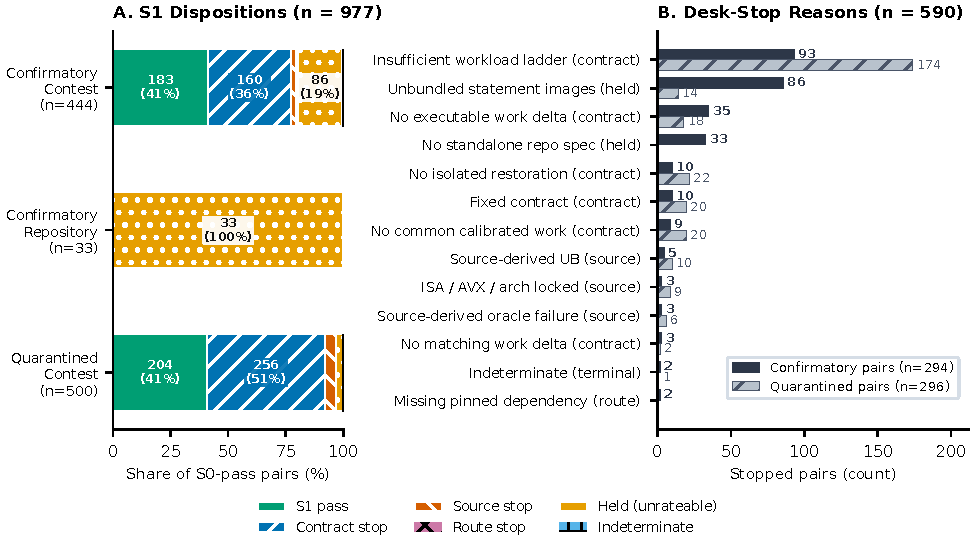
\includegraphics[width=\linewidth]{fig_s1_desk_taxonomy.pdf}
\caption{Verified S1 qualification outcomes across all 977 S0-pass pairs
(96/96 batches sealed; 844 rateable---including 3 terminal
\texttt{indeterminate} judgments under Amendment~4---plus 133 held
\texttt{desk\_unrateable}).
Panel~A shows shares per stratum; Panel~B shows the 590 total S1 stops
split by confirmatory pairs ($n=294$, spanning 293 representative clusters)
vs.\ development-exposed quarantined pairs ($n=296$).}
\label{fig:s1-taxonomy}
\end{figure}

\subsection{Primary outcomes and checks on the growth screen}

The representative execution yield (P1) was \BenchExecRate. The
equal-cluster difference between desk-stop and execution rates (P2) was
\BenchDeskContrast. Among fitted representatives, \BenchFitAlertRate{}
passed the all-stream screen (P3). Relative to intake-passing
representatives, yield was \BenchIntakeAlertRate{}
(Figure~\ref{fig:outcomes-forest}). The cluster counts and
gate determinations were \BenchGates. Unadjusted and Holm-adjusted
test results for the analyses meeting their gates were \BenchTests.
Frame-specific denominators and estimates were \BenchFrames.

\begin{figure}[htbp]
\centering
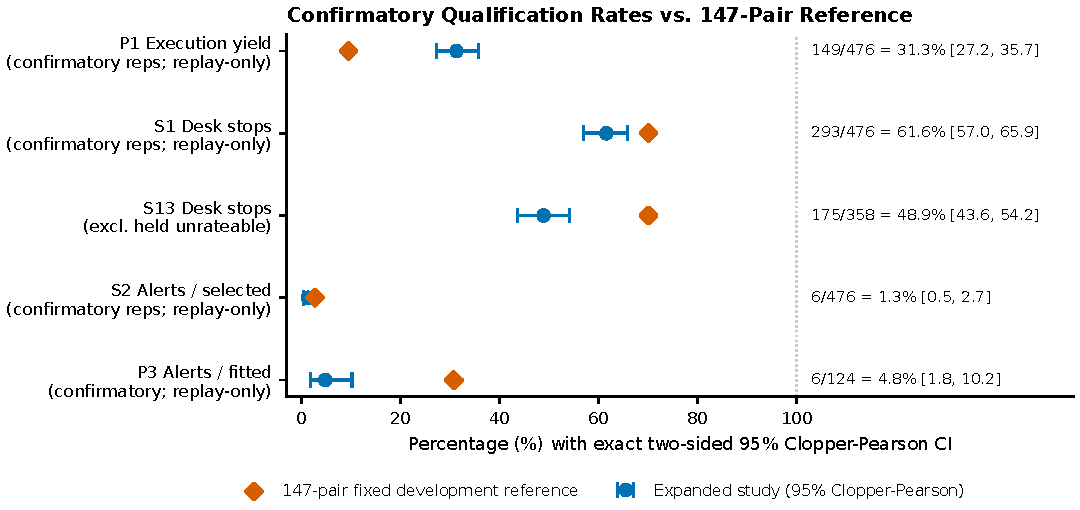
\includegraphics[width=\linewidth]{fig_qualification_outcomes.pdf}
\caption{Confirmatory qualification rates and exact two-sided 95\%
Clopper--Pearson intervals versus the fixed 147-pair development references
(diamonds). P1, P3, and all S1-dependent secondary rates (Sec.~S1, S2, S13)
are \emph{replay-only} under Amendment~3 because S1 labels derive from one
vendor workflow with undisclosed routing; P3 satisfies its $\ge 30$
confirmatory fitted-cluster gate ($n=124$).}
\label{fig:outcomes-forest}
\end{figure}

For the admitted fits, the disposition under the any-stream rule and
drop-largest refit was \BenchFitSensitivity. Variant and censoring checks
showed \BenchVariantChecks. The
infrastructure-exclusion and all-pair sensitivity results were
\BenchPairSensitivity. The separate development-exposed results were
\BenchExposedResults. The native-build decision and its inputs were
\BenchBuildDecision. These comparisons distinguish refusal to make a
claim because the evidence was insufficient from a measured failure to
meet a cutoff.

\subsection{Desk label checks}

Inter-model S1 agreement was not measured (\BenchModelAgreement). The
fixed blind sample yielded a \BenchAuthorCheck. Across the three non-empty primary buckets, the primary
rater's 22 \texttt{pass} decisions split under blind author review into 3
\texttt{pass}, 12 \texttt{contract} stops, and 7 \texttt{source} stops; its
26 \texttt{contract} stops split into 19 \texttt{contract}, 3 \texttt{pass},
and 4 \texttt{source}; and both \texttt{source} stops agreed (2/2). Thus,
disagreement stemmed predominantly from stricter author screening on contract
and source eligibility rather than arbitrary noise, consistent with the
$32/183$ ($17.5\%$) constructive pre-S3 failure rate. We report the author
comparison as a descriptive check on rubric application only; it never
alters primary labels and is no validation of unobserved outcomes of
desk-stopped pairs.

\section{Discussion and threats to validity}

\paragraph{Interpretation.}
The study measures what is possible under a specified set of checks,
rather than adjudicating the correctness of upstream speedup claims.
The two useful reporting questions are how often the study gets an
admissible comparison at all, and what the fitted comparisons show.
Improvement at the sampled sizes can coexist with a flat ratio; a
growth alert can coexist with no demonstrated wall-clock benefit.
Preserving all dispositions makes either a concentrated pathway of loss
or broad feasibility visible. In particular, comparing P2 across all 476
post-intake clusters ($+30.3$~pp, Holm $p = 6.78 \times 10^{-12}$) against
Sec.~S13 excluding the 118 held \texttt{desk\_unrateable} clusters ($+7.3$~pp
across 358 rateable Contest clusters, 95\% cluster bootstrap $-2.8$ to
$+17.0$~pp, nominal exact sign-flip $p = 0.165$ outside the primary Holm
family) shows that the overall desk-stop dominance is heavily driven by
missing self-contained specifications (86 unbundled contest images and all
32 Repository clusters lacking an independent spec), while among rateable
Contest pairs desk stops ($48.9\%$) and isolated execution ($41.6\%$) occur
at comparable scales; meanwhile, across completed observations, count
stability held with zero disagreements across compiler optimization levels
(9{,}794 \texttt{-O0}/\texttt{-O2}/\texttt{-O3} agreements, 0 disagreements,
1{,}294 capped or missing) and sham checks (7{,}349 target--sham agreements,
0 disagreements, 967 capped or missing), and all 6 all-stream alerts ($6/6$)
passed the $\ge 80\%$ restoration recovery check (0 failed), yet
fitted-case all-stream alerts remained rare ($6/124 = 4.8\%$). The
estimates should not be extrapolated from the fitted subset to pairs
excluded by missing evidence.

\paragraph{Construct and internal validity.}
The named operation is a proxy for one part of work, not a complete cost
model. The oracle and sanitizers test specific inputs and enabled checks;
they do not prove that both programs are equivalent on all inputs.
Instrumented runs can still miss another event or a change outside the
counted region. Checking count stability across compiler optimization
levels, comparing restoration and sham, and refitting without the
largest size address separate failure modes; none licenses extrapolation
beyond the measured range. Desk decisions come from one vendor workflow
whose backend routing is undisclosed and may vary across requests; they
may stop viable cases or admit weak contracts, and a single-author blind
check cannot measure variation among multiple human raters.

\paragraph{External and conclusion validity.}
PIE and CodeNet are contest data with overlapping provenance. The
repository snapshot favors projects and commits visible under a bounded
search and its language, date, and wording filters. An isolated build
can reject a pair that would run with project-native dependencies. The
draw and overlap quarantine reduce dependence but cannot rule out
unidentified aliases or templates. Estimates apply to the defined
frames and protocol; they are not estimates for all C++ code. The
archived references are fixed development comparisons, not sampling
distributions. Frame imbalance is complete in execution (0/32 Repository
clusters executed; Repository is reported as counts only under Amendment~1),
so all isolated execution and fitted-case estimates apply solely to Contest
submissions.

\section{Conclusion}

A public slow--fast pair is an input to benchmark qualification, not a
growth benchmark by itself. Under the frozen protocol, the
intake-to-alert yield was \BenchIntakeAlertRate. \BenchConclusionTakeaway{}
The ledger distinguishes documented stops from negative fits, so readers
can see what was measured and which prerequisites ruled out a comparison.
Any positive finding concerns the named work event on the tested range
under the pinned route.

\section*{Data availability and use of AI}

The frozen manifest identifies public upstream versions by pins and hashes.
The artifact is designed to connect the manifest and the dated protocol
to a terminal ledger, representative identifiers, and receipts that
reproduce the reported estimates where the inputs permit it. The artifact
availability statement and evidence classifications are \BenchAvailability.
We do not release locally retained source payloads, private archives,
or raw rater ballots. A receipt-only check, where provided, does not
constitute a fresh execution. No private-only estimate is reported in the
abstract or conclusion.

Generative AI assisted in drafting. Desk judgments are disclosed as
model judgments, separately from deterministic build, oracle, counter,
and statistical checks.
The methods record identifies the applied rubric, protocol amendments,
and pinned procedures to the extent the evidence can be disclosed.

\bibliographystyle{plain}
\bibliography{paired_mechanism}
\end{document}
